\section{Eisengehalt}

\subsection{Arbeitsgrundlagen}

(Siehe Formelsammlung)


\subsection{Durchf\"uhrung}

\subsubsection*{Versuchsanordnung}

Der Eisengehalt in einer Legierung wurde mit verschiedene Messmethoden bestimmt.


\subsubsection*{Messergebnisse}

\begin{center}
    \begin{threeparttable}
        \caption{Gemessene Gr\"ossen}
        \begin{tabular}{ccc}
            \toprule
            Messung & Eisengehalt (\%) & Absoluter Fehler (\%) \\
            \midrule
            1   & 20.3  & 1.2 \\
            2   & 21.9  & 1.3 \\
            3   & 21.1  & 1.1 \\
            4   & 19.6  & 0.8 \\
            5   & 19.9  & 1.3 \\
            6   & 18.0  & 1.3 \\
            7   & 19.4  & 1.0 \\
            8   & 23.2  & 2.0 \\
            9   & 21.6  & 0.8 \\
            \bottomrule
        \end{tabular}
        \begin{tablenotes}
            \small
            \item \textbf{Hinweis:} Daten wurde vom Auftragsdokument kopiert.
        \end{tablenotes}
    \end{threeparttable}
\end{center}

Es soll der einfache sowohl auch der gewichtete Mittelwert berechnet werden. Weiterhin soll auch
der einfache und gewichtete Fehler berechnet werden.


\subsubsection*{Mittelwert}

Der einfache Mittelwert berechnet sich mit der Formel
\begin{equation}
	\bar{x}_{einfach} = \frac{1}{9} \sum_{i=1}^{9} x_i = \SI{20.6}{\percent}
    \label{eq:einfacher-mittelwert}
\end{equation}

wobei $x_i$ das Eisengehalt in Prozent ist.

Der gewichtete Mittelwert l\"asst sich mit der Formel
\begin{equation}
	\bar{x}_{gewichtet} = \frac{ \sum_{i=1}^{9} g_{\bar{x}_i} \cdot x_i}{ \sum_{i=1}^{9} g_{\bar{x}_i}} = \SI{20.4}{\percent}
    \label{eq:gewichteter-mittelwert}
\end{equation}

berechnen, wobei
\begin{equation}
	g_{\bar{x}_i} = \frac{1}{s_{\bar{x}_i}^2}
    \label{eq:gewicht}
\end{equation}

und $x_i$ der Eisengehalt in Prozent ist und $g_{\bar{x}_i}$ der absoluter Fehler in Prozent ist.


\subsubsection*{Fehler}

Der einfache Fehler berechnet sich mit der Formel
\begin{equation}
	s_{\bar{x}_{einfach}} = \sqrt{ \frac{ \sum_{i=1}^{9} (x_i - s_{\bar{x}})^2}{ 9 \cdot (9-1) }} = \SI{0.5}{\percent}
    \label{eq:einfacher-fehler}
\end{equation}

wobei $x_i$ der Eisengehalt in Prozent ist und $s_{\bar{x}}$ der \emph{einfache} Mittelwert ist.

Der gewichtete Fehler berechnet sich mit der Formel
\begin{equation}
	s_{\bar{x}_{gewichtet}} = \frac{1}{ \sqrt{ \sum_{i=1}^{9} g_{\bar{x}_i} } } = \SI{0.4}{\percent}
    \label{eq:gewichteter-fehler}
\end{equation}

wobei $g_{\bar{x}_i}$ wieder mit der Formel \ref{eq:gewicht} berechnet wird.


\subsubsection*{QtiPlot}

\begin{figure}[H]
    \center
    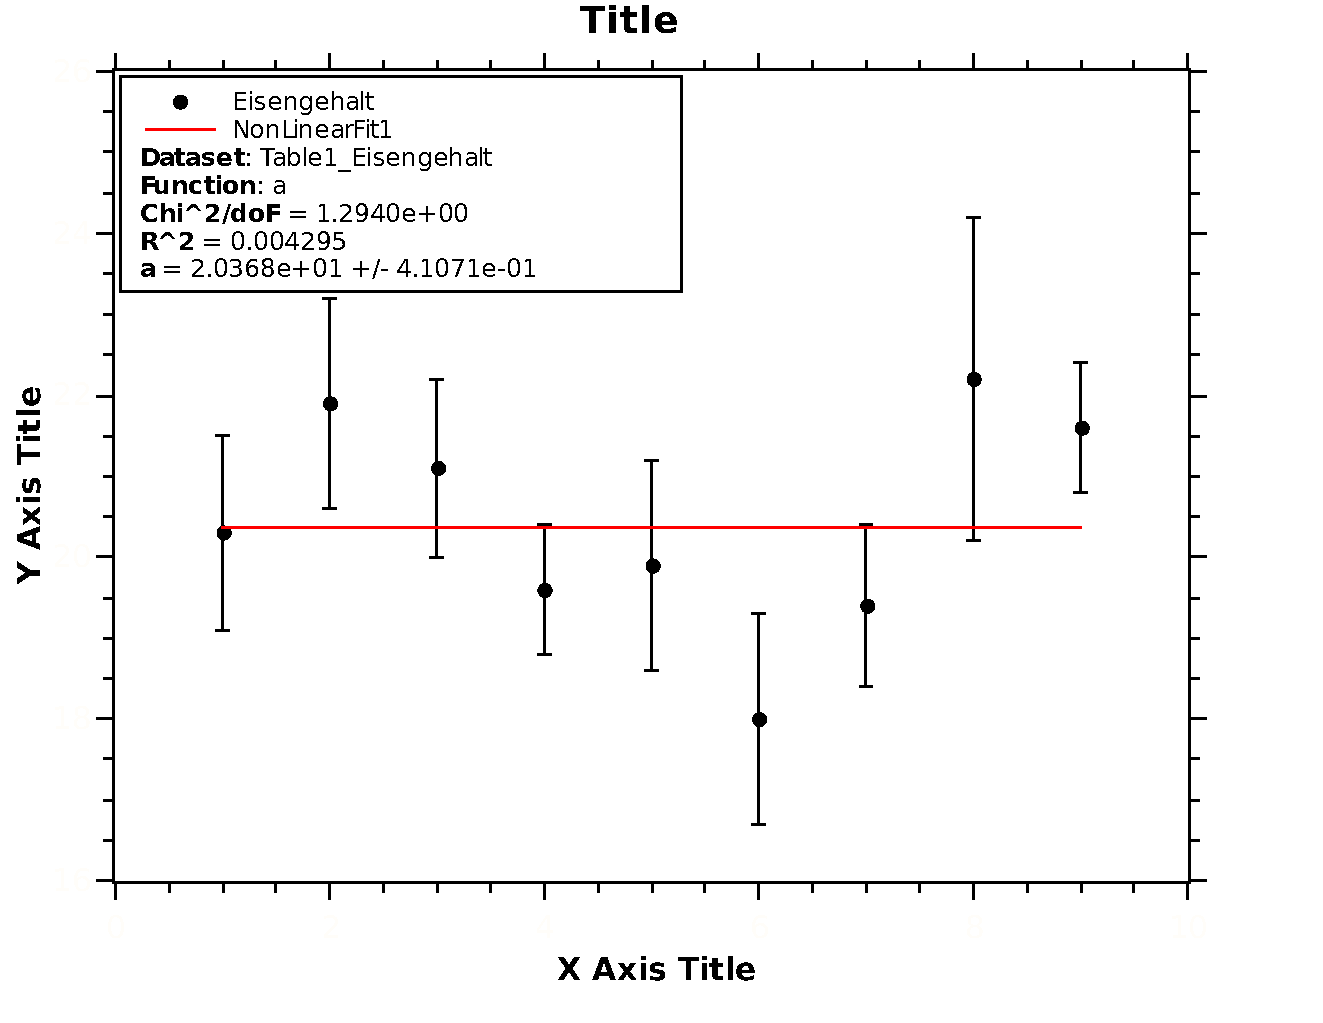
\includegraphics[width=.85\textwidth]{qtiplot/eisengehalt}
    \caption{XY-Scatter der gemessenen Eisengehalte mit Fehler}
    \label{fig:eisengehalt}
\end{figure}


\subsection{Resultate und Diskussion}

Von QtiPlot in der Figur \ref{fig:eisengehalt} kann der berechnete Wert von $a=(20.4 \pm 0.4)\SI{}{\percent}$
ausgelesen werden. Dieser Wert vergleicht sich ganz gut mit den Resultaten der Formeln
\ref{eq:gewichteter-mittelwert} und \ref{eq:gewichteter-fehler} von $(20.4 \pm 0.4)\SI{}{\percent}$.

